\chapter{Deep Learning and Curriculum Learning}
Humans are different from other species in many ways, but two of them are particularly noteworthy. 
First of all, humans display an exceptional capacity to learn;
moreover, humans are remarkable for the long time they take to reach maturity. Human beings need about two decades to be trained as fully functional adults for our society and it may
be argued that, through culture, learning has created the basis for a non-genetically based transmission of behaviors and habits which might
accelerate the evolution of our species. Infancy and childhood are times of great vulnerability for the young, when the first skills are developed and when the adults who
must care for and protect their own young go through a severe restriction of their range of activities. Then, why would evolutionary process not prune a long period of 
immaturity from our species? Previous research carried out by Elman \textit{et al} \cite{ELMAN199371} at the intersection of cognitive science
and machine learning underline that it is important to remember that the evolution looks at the whole individuals rather than at the value of isolated traits; the adaptive success of individuals therefore is 
determined by the joint interaction of all their traits. Thus, it might be that to understand the persistence of one trait with apparently negative consequences - such as the lenghty period of immaturity - possible interactions
with other traits - such as the ability to learn - may need to be considered. The perfect example of such an interaction, is that in human beings the greatest learning occurs precisely in the period of time
when they are undergoing major changes, during childhood indeed.\\
In humans, learning and development interact in a way that is as important as non-obvious; maturational changes might provide the enabling 
conditions which allow learning to be most effective.
It is a matter of fact that the higher the training is organized, the better the knowledge of the person. Humans in fact learn much better when the examples are not randomly presented, but organized in such a way 
where the amount of concepts is incremented gradually, and where the complexity of them increases over time. The majority of education systems are organized in order to illustrate 
different concepts at different times, exploiting previously learned notions to ease the learning of new abstractions. By choosing which examples to present and in which order to explain them to the learning system, one can guide
training and consequently increase the speed at which learning can happen. This is the same idea exploited in \textit{animal training} by psychologists Skinner (1958), Peterson (2004) and Krueger \& Dayan (2009)
where it is called \textit{shaping}.
In the context of machine learning, such a meaningful learning process is known as \textit{curriculum learning}.

\section{State of the art}
The basic idea of \textit{curriculum learning} - traced back to Elman - is to start small, learn easier aspects
of the task, and then gradually increase the difficulty level.
Inspired by human learning in fact, curriculum learning (CL) is a training strategy that emphasizes
the order of training instances in a computational learning setup.
As a feature of human learning, curriculum - or even better learning in a meaningful way -
has been transferred to machine learning, thus creating the subdiscipline named
\textit{curriculum learning}.
Essentially, human education is organized as curricula, by starting small indeed, and gradually presenting more complex
concepts. The paramount hypothesis is that simpler instances should be learned
during the first steps as building blocks, to then learn more complex ones. Several experiments on sentiment 
analysis task and tasks similar to sequence prediction tasks in NLP carried on by Cirick \textit{et al} \cite{Cirik2016VisualizingAU} prove that
curriculum learning has positive effects on LSTM's internal states, by biasing the model through building constructive representations. 
Specifically, the internal representation at the previous timestep is used as building block for the next one, thus
contributing at the final prediction.\\
In traditional machine learning algorithms all the training examples are randomly presented to the model,
thus ignoring the different complexities of data instances and the learning status of the current model. 
Owning to this, it is fairily intuitive wondering if the curriculum training strategy could ever benefit machine learning.
Extensive experiments from early \cite{bengio2009curriculum}, \cite{kumar2010self}, \cite{zaremba2014learning} to recent works \cite{fan2018learning}, \cite{graves2017automated}, \cite{hacohen2019power}, \cite{platanios2019competence} in various applications of machine learning show that such strategy is of benefit to this field, but not always, and 
because of that the power of introducing the curriculum-like strategy depends on how the curriculum for specific applications and datasets are designed.

\section{Curriculum Learning related works}
As the idea of CL provide a general training strategy beyond specific machine learning
tasks, its power have been exploited in considerably wide application scopes, including supervised learning
tasks within computer vision \cite{guo2018curriculumnet}, \cite{jiang2014easy}, natural language processing (NLP) \cite{platanios2019competence}, \cite{tay2019simple}, healthcare prediction \cite{el2020student}, various
reinforcement learning (RL) tasks \cite{florensa2017reverse}, \cite{narvekar2017autonomous}, \cite{ren2018self} as well as other applications such
as graph learning \cite{gong2019multi}, \cite{qu2018curriculum} and neural architecture search (NAS) \cite{guo2018curriculumnet}. As already mentioned in \ref{chapter:MAO}, the advantages of applying CL
training strategies to miscellaneous real-world scenarios can be mainly summarized as (i) improving the model performance on 
target tasks, and (ii) accelerating the training process, which cover the two most significant 
requirements in most of the machine learning research. \\
For instance,
Platanios \textit{et al.} \cite{platanios2019competence} present 
a personal framework that consists of a way of deciding which training instances
are shown to the model at different times during training, based on 
an estimated difficulty of a sample and on the current competence
of the model. Thus, filtering training samples prevents the model from 
getting stuck in bad local optima, making it converge faster and reach
a better solution than the common approach of uniformly 
sampling training examples. Their experiment shows that CL helps the 
neural machine translation model reduce training time by up to 70\%, while at the 
same time obtaining accuracy improvements of up to 2.2 BLEU points, compared
to plain training without any curricula. \\ To further illustrate, in \cite{florensa2017reverse} Florensa 
\textit{et al.} talk about curriculum learning as a reverse curriculum technique. 
They propose a method to learn goal-oriented tasks without requiring
any prior knowledge, other than obtaining a single state in which
the task is achieved. They dimonstrate that their approach is 
based on a reverse training, where the robot gradually learns to reach 
the goal from a set of start states increasingly far from the goal.
That approach resulted in solving hard problems, not solvable 
by state-of-the-art reinforcement learning methods.

\section{Curriculum Learning application in Deep Learning tasks}
Training neural networks is traditionally done by providing a sequence of 
random mini-batches sampled uniformly from the entire training data. Conversely, curriculum learning
involves the non-uniform sampling of mini batches, on the training of deep networks.
However, understanding why and when \textit{starting small} strategies can 
benefit machine learning algorithms is a question that every scholar try to contribute to.
Bengio \textit{et al.} \cite{bengio2009curriculum} other than showing several cases where very simple
multi-stage curriculum strategies give rise to improved generalization and faster convergence, 
contribute to the question introducing a hypothesis which might help to explain 
some of the advantages of a curriculum strategy. They argue that a well chosen curriculum 
strategy can act as a continuation method. Intuitively, continuation methods are optimization
strategies for non-convex criteria which first optimize a smoother and easier version of the problem to 
reveal the "global picture", and then gradually consider less smoothing versions, until the target objective of 
interest. Therefore, continuation methods provide a sequence of optimization objectives, starting with an objective for which
it is easy to find a global minimum, and tracking the local minima throughout the training. In this way, continuation methods
guide the training towards better regions  and the local minima learned from easier objectives have better
generalization ability and are more likely to approximate global minima.
To test this hypothesis, they turn the attention to the training of deep
architectures, which have been shown to involve good solutions in local minima that are almost impossible to find 
by \textit{random initialization}. Generally, deep learning methods try 
to learn feature hierarchies, i.e., features at higher levels are formed by the composition of lower level features.
As a consequence, automatically learning multiple levels of abstracion may allow a system to induce complex functions mapping the input to the 
output directly from data, without depending heavily on human-crafted features.
One possible theoretical motivation for deep architectures comes from complexity theory. Some functions, in fact, can 
be represented with an architecture of depth \textit{k} but require an exponential size architecture when the depth 
is restricted to be less than \textit{k}. Training deep networks, however, involves a potentially 
intractable non-convex optimization problem \cite{bengio2009curriculum}. There were no good algorithms for training 
fully-connected deep architectures before 2006, when Hinton introduced a learning algorithm that greedily trains one layer at a time, exploiting an unsupervised
generative learning algorithm for each layer. It is conceivable that by training 
each layer one after the other, the network is organized in such a way that it can first learn the simpler
concepts, represented in the first layer indeed, then sligthly more abstract ones, represented in the second layer, and so on.
Not long after, strategies for building deep architectures from related variants were proposed %add ref 
and these works showed the advantage of those frameworks over shallow ones, and of the unsupervised 
pre-training strategy in a variety of settings.\\

\section{Definition of Curriculum Learning}\label{chapter:defCL}
Based on all the previous works in the first place provided in behavior and 
cognitive science literature, the concept of CL was first proposed in \cite{bengio2009curriculum} with 
experiments on supervised visual and language learning tasks, exploring when and why curriculum could benefit machine learning.
The original definition of CL refers to a curriculum as a sequence of training criteria 
over \(T\) training steps \( C = \left \langle Q_1, ..., Q_t, ..., Q_T \right \rangle\), where each  
criterion \(Q_t\) is a reweighting of the target training distribution \(P(z)\): \(Q_t(z) \propto W_t(z)P(z)\), for 
each instance in the training set.\\ In the definition the following three conditions were considered:
\begin{itemize}
    \item the entropy of distributions gradually increases, \(H(Q_t) < H(Q_{t+1})\);
    \item the weight for any example increases, \(W_t(z) \leq W_{t+1}(z),  \forall z \in D\);
    \item \(Q_T(z) = P(z)\).
\end{itemize}
So, curriculum learning is the training strategy that trains a machine learning model
with a curriculum. The first of the above conditions means that the diversity 
and the information of the training set should gradually increase. More specifically,
the reweighting of examples in later steps increases the probability of sampling slightly more difficult examples.
The second condition instead means to gradually add more training examples, letting the size of the training set increase. 
Finally, the last condition
means that the reweighting of all examples is uniform and the training is carried on the target training set.\\
At a more abstract level, a curriculum can be seen as a sequence of instance selection or example reweighting along the training process in order to achieve faster convergence or better generalization, 
which is beyond the "easy to hard" or "starting small" principles. 

\section{A general CL framework}
In a nutshell, curriculum learning means "training from easier data to harder data" \cite{Wang2020}. More specifically the
core idea is to "start small" \cite{ELMAN199371}, train the machine learning model with easier subtasks, to then gradually increase
the difficulty level of subtasks until the whole training dataset is used.\\
Bearing in mind the strategy of training from easier to harder data, to design such a curriculum idea 
(i) what kind of training data is supposed to be easier than other data, (ii) and when is appropriate to present more harder
data for training - and how much more - must necessarily be decided.
Technically, those two issues can be abstracted as the concepts of a Difficulty Measurer, that decides the "easiness"
of each data instance to start the training process from, and a Training Scheduler, that rules the sequence of data subsets during 
the whole training process \cite{Wang2020}.
Therefore, Difficulty Measurer together with Training Scheduler constitute a general framework for curriculum design,
as illustrated in Figure ~\ref{fig:CLdesign}.
\begin{figure}[h]
    \begin{center}
        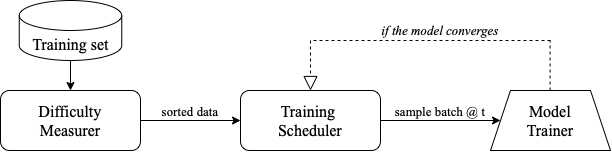
\includegraphics[width=0.55\textwidth]{/Users/carmenarmenti/Desktop/Thesis document/images/predefinedCL.png}
        \caption{\label{fig:CLdesign}Predefined Curriculum Design.}
    \end{center}
\end{figure}
First of all, the Difficulty Measurer sorts all the training examples from the easiest 
to the hardest and passes them to the Training Scheduler. Then, at each training epoch \textit{t}, the Training Scheduler
samples a batch of training instances from the easier subset and gives them to the Model Trainer for training.\\
As training epochs increase, the Scheduler decide when to sample from more harder data, generally until uniform sampling
from the whole training set. This schedule either depends on the training loss feedback from the Model Trainer, or on some other
parameters that implies that the model would deverge, if left to training for more epochs.\\
Moreover, a distinction between \textbf{predefined CL} and \textbf{automatic CL} must be clarified. The first refers to the framework
where both the Difficulty Measurer and Training Scheduler are defined by human prior knowledge, thus with no data-driven
algorithms involved; the latter instead, if any - or both - of the components are designed by data-driven algorithms.\\
Usually, the power of introducting Curriculum into Machine Learning depends on how the curriculum for specific
applications and dataset is designed. Due to this, Difficulty Measurers often relies on the data
characteristics of specific tasks, and most of them are defined by a definition of complexity, diversity, or noise estimation.

\subsection{Predefined Curriculum Learning}
\label{subsection:predCL}
To begin with, the \textit{difficulty measurer} depends on the data characteristics, and consequently
on the specific task. 
By and large, common types of difficulty measurers are designed for image and text data, as usually happens in computer vision and natural language processing tasks, 
but also for other data types such as audio data and programs. 
As we mentioned before, difficulty measurers can rely on data complexity, diversity, or noiseness.
In the first place, \textit{complexity} refers to the structural complexity of a data example, in a way that the higher the complexity, 
the harder for the model is to capture the samples. 
Some of the most popular difficulty measurers are: the \textit{sentence length} - the most used in NLP tasks;
the \textit{parse tree depth} - where the complexity is based on the grammar; the \textit{nesting operations} in a program - that computes the complexity based on the number of instructions in
program execution tasks. 
As for \textit{diversity}, the distributional diversity of elements in a group data is meant to define a type of difficulty measurer.
The more various the data, the harder the learning process is.
When more - or rare - types of data is included in the training data set, training is more difficult for the model. 
One of the most used measure of diversity is information entropy, which in text data is exploited as the Part-Of-Speech (POS) entropy. One other measure is the word rarity.
Last but not least, another definition of difficulty is the \textit{noise extimation}, which estimates
the noise level of data examples and classifies cleaner data as easier. To provide an illustration, in \cite{chen2015webly}
the authors present an approach to train a webly supervised convolutional neural networks (CNN), inspired by curriculum learning.
They suppose that images retrieved by a search engine like Google are supposed to be cleaner, thus easier, while images
posted on photo-sharing website like Flickr are more realistic, therefore noiser and consequently harder. 
So, examples with lower local density are considered to be harder to predict. 
On top of that, there are also other difficulty measurers that rely on 
characteristics such as signal intensity or humanly-annotated image difficulty scores.
\newline
If predefined difficulty measurers vary over different data types and tasks, on the other hand
the existing predefined \textit{training scheduler} are usually independent from the data - and then from the task.
However, training schedulers can be differentiated as well; they are usually divided into \textit{discrete} and \textit{continuous} schedulers.
Discrete schedulers adjust the training data subset following a specific criterion - 
be it a fixed number of epochs or the convergence on the current data subset - whereas continuous schedulers adjust 
the training data subset at every epoch.
Thanks to their semplicity and effectiveness \textit{discrete schedulers} are widely adopted and the most popular
discrete scheduler is named as \textit{Baby Step}. 
\begin{algorithm}
    \caption{Baby Steps Curriculum \cite{cirik2016visualizing}, \cite{wang2021survey}}\label{alg:bbstep}
    \hspace*{\algorithmicindent} \textbf{Input}: \text{\(\mathbf{C}\): training dataset; \(\mathbf{D}\): Difficulty Measurer;}\\
        %\mathit{D:} the Training Dataset; \mathit{C:} the Difficulty Measurer;\\
    \hspace*{\algorithmicindent} \textbf{Output}: \text{\(\mathbf{M^*}\): optimal model.}
        %\mathbold{M^*:} the optimal model. 
    \begin{algorithmic}[1]
    %\Require \mathit{D: the Training Dataset;} \mathit{C: the Difficulty Measurer;}
    %\Ensure \mathbold{M^*}
    \State $D'= sort(D,C);$
    \State $\lbrace D^1, D^2,...,D^k \rbrace = D'$ where $C(d_a) < C(d_b)$, $d_a\in D^i$, $d_b\in D^j$, $\forall i<j;$
    %$d_a\inD^i$, $d_b\inD^j$, \forall $i<j$
    \State $D^{train} = \emptyset$
    \For{$s = 1$ to $k$}
        \State $D^{train} = D^{train} \cup D^s;$
        \While{not converged for \textit{p} epochs}
        \State train$(M, D^{train});$
        \EndWhile
    \EndFor
    \end{algorithmic}
\end{algorithm}
\newline
Algorithm~\ref{alg:bbstep} first distributes the sorted data into buckets - from easy to hard - and starts training with the easiest one, 
shuffling the current buckets and the data in each bucket and sampling mini-batches for training.
Then, when convergence is reached or after a defined number of epochs, the next bucket is merged in the current one. 
This process continues until all the buckets are merged in one unique training set; at this point the training process either stops or continues 
several extra epochs. \\
Another discrete scheduler is called \textit{One-Pass} which uses a similar strategy for data bucketing and for starting the training from the easiest one;
however, if Baby Step merges the buckets as soon as the model converged on the previous bucket, One-Pass scheduler when updating the training data discards the current bucket
and switches to the next harder one. 
\begin{algorithm}
    \caption{One-Pass Curriculum \cite{cirik2016visualizing}}\label{alg:onepass}
    \hspace*{\algorithmicindent} \textbf{Input}: \text{\(\mathbf{C}\): training dataset; \(\mathbf{D}\): Difficulty Measurer;}\\
        %\mathit{D:} the Training Dataset; \mathit{C:} the Difficulty Measurer;\\
    \hspace*{\algorithmicindent} \textbf{Output}: \text{\(\mathbf{M^*}\): optimal model.}
        %\mathbold{M^*:} the optimal model. 
    \begin{algorithmic}[1]
    %\Require \mathit{D: the Training Dataset;} \mathit{C: the Difficulty Measurer;}
    %\Ensure \mathbold{M^*}
    \State $D'= sort(D,C);$
    \State $\lbrace D^1, D^2,...,D^k \rbrace = D'$ where $C(d_a) < C(d_b)$, $d_a\in D^i$, $d_b\in D^j$, $\forall i<j;$
    %$d_a\inD^i$, $d_b\inD^j$, \forall $i<j$
    \For{$s = 1$ to $k$}
        \While{not converged for \textit{p} epochs}
        \State train$(M, D^{train});$
        \EndWhile
    \EndFor
    \end{algorithmic}
\end{algorithm}
\newline
One-Pass is less used than Baby Step in curriculum learning literature due to the lower performance in many tasks.
In fact, the complexity or diversity of the training data if gradually increasing
helps improve generalization - as happens in Baby Step scheduler; on the other hand,
One-Pass scheduler (see Algorithm~\ref{alg:onepass}) is like training on a sequence of independent tasks as in 
continual learning - which faces the problem of forgetting even though the early tasks are easier 
(we also faced this issue as we explain in Chapter~\ref{chapter:chap4}).
Other discrete schedulers are also based on data bucketing, but take 
different sampling strategies. For example, some \cite{kocmi2017curriculum} modify the Baby Step to unevenly divide 
the examples into buckets such that easier buckets have more data examples; then they sample instances
without replacement from the easiest bucket only until there remain the same number of 
examples as in the second easiest bucket. Afterward, they uniformely sample 
from the first two buckets until the size is the same as that of the third bucket.\\
In \cite{zaremba2014learning} instead, the researchers base their experiments on two measures to 
define a difficulty measurer: \textit{length} and \textit{nesting} of a dataset of programs.
They evaluate four different curriculum learning strategies, two of which proved to be better than using no curriculum strategy or the 
naive curriculum strategy - the latter was tested in \cite{bengio2009curriculum} as well.
The first of the two approaches - both successful in the context of evaluating 
short computer programs - is a \textit{mixed strategy} where the training samples
are picked randomly over a set of random lengths \([1, a]\) and random nestings \([1, b]\),
thus using a balanced mixture of easy and difficult examples at every point during training.
The second one instead is a \textit{combined strategy} between the naive curriculum strategy 
and the mixed strategy. In this approach, every training case is obtained 
either by the naive method or by the mixed one. 
Thence, the combined strategy always exposes the network at least to some difficult examples, which is the key element 
in which it differs from the naive curriculum strategy. As explained in their 
piece of work, both their curriculum strategies outperform the naive curriculum strategy, especially 
the combined one, in a matter of hidden state allocation.\\
\textbf{Predefined CL limitations.} Even if predefined curriculum learning is simple and effective, there are 
some limitations in terms of (i) applicability, (ii) difficulty measurer definition, (iii) training scheduler definition.
First of all, an expert domain knowledge is needed not only to find the most suitable
combination of difficulty measurer and training scheduler for a specific task and its dataset, 
but also for designing both of them in such a way that are predefined before the training starts.
Moreover, defining a predefined difficulty measurer means humanly decide what should be the difficulty boundaries of a model - which are
different from those of humans. Finally, when a training scheduler remains fixed 
it is not flexible enough, since it ignores the feedback of the current model to some extent.
On top of the previous, the best hyperparameters of training scheduler are hard to find and there are no 
other methodologies other than exhaustive trials. In addition, taking Baby step as example, 
a basic problem in its scheduler is the decision of the number of buckets and how to divide them. In fact, 
deciding by thresholds on difficulty scores makes it hard to assign each bucket with roughly the same number of instances; on 
the other hand, division by size might result in fluctuations in difficulty within a bucket or not enough difference between different 
buckets.\\
\newline
These limitations of predefined curriculum learning has led to the development 
of more data-and-model-driven approaches rather than human-driven, in such a way 
that they can be more dynamically adaptive to the training in process: automatic 
CL approaches.

\subsection{Automatic Curriculum Learning}
The automatic curriculum learning approaches try to break the limits of predefined curriculum learning approaches.
Taking as reference the issues mentioned before, i.e., (i) applicability, (ii) difficulty measurer definition, and (iii) training scheduler definition, 
by and large it can be said that: (i) in terms of \textit{applicability} automatic CL strategies 
tend to be general and domain agnostic; (ii) \textit{difficulty measurers} are model decided thus dynamic; (iii) \textit{training schedulers}
are dynamically defined and redefined by model feedbacks.\\
In predefined CL who designs the curriculum is a human expert, whereas the entity that is trained
by the curriculum is the machine learning model, metaphorically the two parties can be referred as 
a \textit{teacher} and a \textit{student}. So, automatic CL is meant
to reduce the need for \textit{human} teachers, and in \cite{wang2021survey} the authors summarize 
four methodologies of predefined CL that take different ideas, among all the ideas.

Firstly, \textbf{Self-paced Learning} (SPL) is a primary branch of CL that automates the Difficulty Measurer
by taking the example-wise training loss of the current model as criteria. The SPL methods let the students themselves
act as the teacher and measure the difficulty of training examples according to its losses on them. 
This concept is analogous to the self-study human approach, in fact
originates from human education, where the student can control the learning curriculum, including what, how, when, and how long 
to study. In machine learning context, SPL refers to a training strategy - initially proposed by Kumar \textit{et al.} \cite{kumar2010self} -
which trains the model at each iteration with the proportion of data with the lowest training losses.
Such a proportion of easiest examples gradually increase until the whole training set is considered, so using a predefined Training Scheduler.
Even if in the literature of SPL CL and SPL are usually mentioned as two different strategies - where the CL 
refers to the predefined CL - in the piece of work aforemetioned SPL is considered as a branch of automatic CL, since it shares 
the spirit with CL and fits with the general framework as explained by Kumar \textit{et al.} in \cite{kumar2010self} and shown in Figure~\ref{fig:SPL-CL}.
\begin{figure}[h]
    \begin{center}
        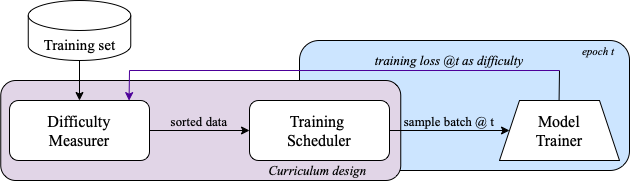
\includegraphics[width=0.55\textwidth]{/Users/carmenarmenti/Desktop/Thesis document/images/SPL-CL.png}
        \caption{\label{fig:SPL-CL}Automatic CL: Self-paced Learning Design.}
    \end{center}
\end{figure}
The most valuable advantages of SPL over predefined CL are twofold: (i) SPL is semi-automatic CL 
with a loss-based automatic Difficulty Measurer and dynamic curriculum, which makes the strategy more flexible and adaptive for various tasks; (ii) SPL includes the curriculum
design into the learning objective of the original machine learning tasks, thus making it applicable as a tool.\\
The authors in \cite{wang2021survey} also specify that other than the original version of SPL, there also exist not only theories for the 
convergence, robustness and essence of SPL to support applications, but also enhanaced versions from different 
perspectives. Moreover, they argue that as a student-driven weighting strategy on the learning objective, the core 
design of SPL is the Self Paced regularizer, which directly determines the optimal weights at each training epoch. Therefore,
most of the existing improvements on SPL have been focused on SPL regularizers. Without going into details, they differentiate (i) Soft SP-regularizers, 
comparing them to Hard Regularizers; (ii) Prior-embedded SPL, and (iii) other enhancements of SPL.

Secondly, there exists a reliable teacher-driven difficulty strategy, that is the \textbf{Transfer Teachers} approach.
SPL takes the current student model as an automatic Difficulty Measurer, however, this strategy has a risk of uncertainty at the beginning of the training, when the student model
is not sufficiently trained. As happens in human education in fact, if students understand 
little about - or misunderstand - the learning materials, it would be hard for them to measure the difficulty of the materials 
and find out the easy ones. So, an idea is to ask a mature tacher for help: an educated person can assess
the materials and form an easy-to-hard curriculum. This idea leads the CL approaches to the Transfer Teachers strategy (see Figure~\ref{fig:TT-CL}).
\begin{figure}[h]
    \begin{center}
        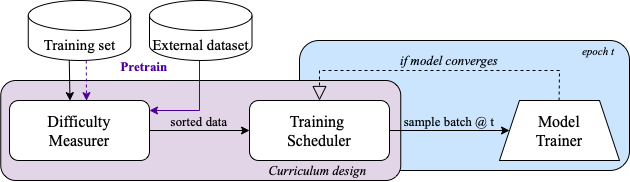
\includegraphics[width=0.55\textwidth]{/Users/carmenarmenti/Desktop/Thesis document/images/TT-CL.png}
        \caption{\label{fig:TT-CL}Automatic CL: Transfer Teacher Learning Design.}
    \end{center}
\end{figure}
The latter is a semi-automatic method that first pretrains a teacher model on the training datasat or an external dataset, ad then transfers its knowledge
to compute the example-wise difficulty, based on which a predefined Training Scheduler can be applied to finish the CL design. 
Transfer Teachers can be helpful to the tasks where the example-wise eaasiness is hard to define.
The most general Transfer Teachers are loss-based, thus they do not need any domain knowledge and are closely related 
to SPL. Concretely, these methods take the example-wise losses calculated by a teacher model as the example difficulty 
and assume that the lower the loss, the easier the example. The teacher model can either be different 
from the student model \cite{weinshall2018curriculum} - so being more complex, or share the same structure with it \cite{hacohen2019power}, \cite{xu2020curriculum}.

Then, \textbf{Reinforcement Learning (RL) Teacher} methods are exposed, which involve a student model and a reinforcement-learning-based 
teacher model. The SPL and Transfer Teacher only automate the Difficulty Measurer and still use predefined
Training Scheduler, thus they only consider one side of the \textit{curriculum} or \textit{teaching} scenario. On one hand
SPL taked the student feedback, i.e., the losses to adjust the curriculum, whereas Transfer Teacher leverages the teacher's knowledge
to determine the order of presenting learning materials. However, in a common and ideal human-based education a teaching strategy
usually involve both the teacher and the student, where the student can interactively provide feedback to the teacher, and the teacher 
can adjust the teaching action accordingly. By doing so, the teacher and the student make progress together.
Even if this strategy costs more than SPL and Transfer Teacher, is the most flexible and completely automatic.
\begin{figure}[h]
    \begin{center}
        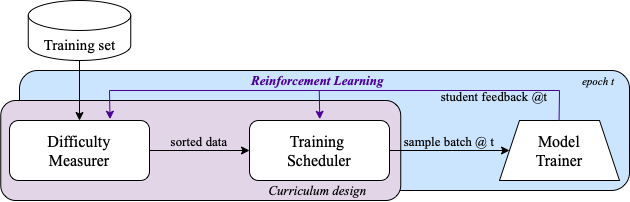
\includegraphics[width=0.55\textwidth]{/Users/carmenarmenti/Desktop/Thesis document/images/RLteacher-CL.png}
        \caption{\label{fig:RLteacher-CL}Automatic CL: Reinforcement Learning teacher Design.}
    \end{center}
\end{figure}
As can be seen in Figure~\ref{fig:RLteacher-CL}, it is clear that with the teacher-student interactive
stratey, RL Teacher achieves the fully-automated CL design. At each training epoch, the RL teacher
will dinamically select examples for training according to the student feedback. The RL Teacher 
sets the teacher model as both the Difficulty Measurer and Training Scheduler by dynamically considering 
the student feedback.\\
On top of that, RL Teacher methods make it possible to set different student feedback according 
to different goals, in fact, they are also suitable for multi-tasking learning, where the teacher model 
selects the most valuable tasks for the student training. Some examples are AutoCL \cite{graves2017automated} and TSCL \cite{matiisen2019teacher}, and for both of them the goal is 
to learn a student model that achieves high performance on all the tasks.

Finally, the scholars report \textbf{other Automatic CL} approaches. In fact, besides RL Teacher,
there exist some other fully-automatic CL designs. These designs should require the generation of the 
curriculum to rely only on the dataset, the student model, and the goal of the task.
Thus, accordingly to this idea and recalling the CL definition in Section~\ref{chapter:defCL}, from the optimization
perspective the authors summarize that the objective is optimize the mapping between the data, the current state 
of the student model, the task goal, and the training goal. To this end, RL Teacher methods typically adopt a RL framework to learn 
the policy for data selection, but as the authors report, there are more optimization methods 
such as Bayesian Optimization, Stochastic Gradient Descent, Meta-learning, and Hypernetwork, which also demonstrated to have great potential to learn 
this mapping.\\
\newline
To sum up, even though there are a lot of different CL methodologies, there is no systematic conclusion 
with regard to how to choose among them in real-world applications. One useful principle for selecting 
a proper CL category is to consider how much prior knowledge one have about the dataset and the task goal.
If sufficient expert domain knowledge is available, then predefined CL methods are more preferable to design a \textit{knowledge-driven} curriculum 
specifically suitable to the exact scenario. On the other hand, if there is no prior assumptions on the data, then 
automatic CL methods are more prefereable to learn a \textit{data-driven} curriculum adaptive to the underlying dataset and task goal.
%%%%%%%%%%%%%%%%%%%%
% NOTES
% As mentioned previously, this is the first work studying LSTM networks
% on software engineering tasks with curriculum learning to our knowledge.

%%%%%%%%%%%%%%%%%%%%